%%%%%%%%%%%%%%%%%%%%%%%%%%%
\usepackage{tikz}
\usetikzlibrary{shapes.geometric}
\usetikzlibrary{calc}
\newcommand{\tikzsetup}{
  \tikzstyle tikzdefault=[semithick,>=stealth];
  \tikzstyle dotnode=[fill,circle,inner sep=1pt];
  \tikzstyle morphism=[circle,draw,inner sep=1pt, minimum
size=18pt, scale=0.8];
  \tikzstyle coupon=[draw,inner sep=1pt, minimum size=18pt,scale=0.8];
  \tikzstyle overline=[preaction={draw,line
width=2mm,white,-},semithick,>=stealth];
  \tikzstyle drinfeld center=[>=stealth,green!60!black, double
distance=1pt]];
  \tikzstyle cell=[fill=black!10,draw, very thin];
   \tikzstyle midarrow=[fill, dart, dart tail angle=112,
    dart tip angle=53,inner sep=0.55pt,sloped,allow upside down];
   \tikzstyle revmidarrow=[fill, dart, dart tail angle=112,
    dart tip angle=53,inner sep=0.55pt,sloped,
    allow upside down,rotate=180];
}
%%%%%%%%%%%%%%%%%%%%%%%%%%%
\newcommand{\OrientedCircle}[1][]{
  \begin{scope}[tikzdefault,#1]
  \draw[->] (-1,0) arc (-180:0:1);
  \draw[-] (1,0) arc (0:180:1);
  \end{scope}
}
%%%%%%%%%%%%%%%%%%%%%%%%%%%
\newcommand{\HalfDashedCircle}[1][]{
  \begin{scope}[tikzdefault,#1]
  \draw[densely dashed, -] (0,1) arc (90:270:1);
  \draw (0,-1) arc (-90:90:1);
  \end{scope}
}
%%%%%%%%%%%%%%%%%%%%%%%%%%%
\newcommand{\HalfDashedOrientedCircle}[1][]{
  \begin{scope}[tikzdefault,#1]
 \draw[densely dashed, -] (0,1) arc (90:270:1);
  \draw[->] (0,-1) arc (-90:0:1); 
  \draw[-] (1,0) arc (0:90:1);
   \end{scope}
}
%%%%%%%%%%%%%%%%%%%%%%%%%%%
\newcommand{\tzRoundCouponI}{
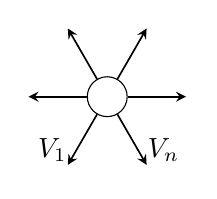
\begin{tikzpicture}[baseline=0pt]
\tikzsetup
\node[morphism] (ph) at (0,0) {$\ph$};
\draw[tikzdefault,->] (ph)-- +(240:1cm) node[pos=0.7, left] {$V_1$} ;
\draw[tikzdefault,->] (ph)-- +(180:1cm);
\draw[tikzdefault,->] (ph)-- +(120:1cm);
\draw[tikzdefault,->] (ph)-- +(60:1cm);
\draw[tikzdefault,->] (ph)-- +(0:1cm);
\draw[tikzdefault,->] (ph)-- +(-60:1cm) node[pos=0.7, right] {$V_n$};
\end{tikzpicture}
}

%%%%%%%%%%%%%%%%%%%%%%%%%%%
\newcommand{\tzRoundCouponII}{
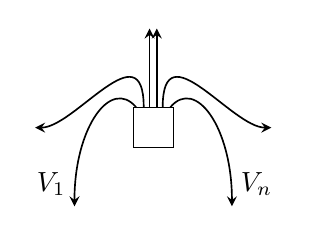
\begin{tikzpicture}[baseline=0pt]
\tikzsetup
\node[coupon] (ph) at (0,0) {$\ph$};
\draw[tikzdefault,->] (ph.130).. controls +(130:0.5cm) and +(90:1cm) ..
                  (-1,-1) node[pos=0.9, left] {$V_1$} ;
\draw[tikzdefault,->] (ph.115).. controls +(90:1cm) and +(0:0.5cm) ..
                  (-1.5,0) ;
\draw[tikzdefault,->] (ph.100) -- +(0,1cm);
\draw[tikzdefault,->] (ph.80) -- +(0,1cm);
\draw[tikzdefault,->] (ph.65).. controls +(90:1cm) and +(180:0.5cm) ..
                  (1.5,0) ;
\draw[tikzdefault,->] (ph.50).. controls +(50:0.5cm) and +(90:1cm) ..
                  (1,-1) node[pos=0.9, right] {$V_n$} ;
\end{tikzpicture}
}
%%%%%%%%%%%%%%%%%%%%%%%%%%%
\newcommand{\tzSummationConventionI}{
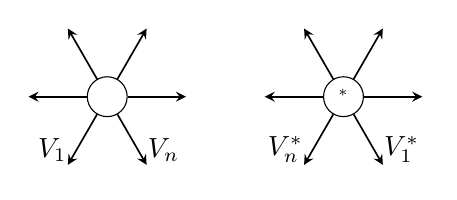
\begin{tikzpicture}[baseline=0pt]
\tikzsetup
\node[morphism] (ph) at (0,0) {$\ph$};
\draw[tikzdefault,->] (ph)-- +(240:1cm) node[pos=0.7, left] {$V_1$} ;
\draw[tikzdefault,->] (ph)-- +(180:1cm);
\draw[tikzdefault,->] (ph)-- +(120:1cm);
\draw[tikzdefault,->] (ph)-- +(60:1cm);
\draw[tikzdefault,->] (ph)-- +(0:1cm);
\draw[tikzdefault,->] (ph)-- +(-60:1cm) node[pos=0.7, right] {$V_n$};
%
\node[morphism] (ph') at (3,0) {$\ph^*$};
\draw[tikzdefault,->] (ph')-- +(240:1cm) node[pos=0.7, left] {$V_n^*$} ;
\draw[tikzdefault,->] (ph')-- +(180:1cm);
\draw[tikzdefault,->] (ph')-- +(120:1cm);
\draw[tikzdefault,->] (ph')-- +(60:1cm);
\draw[tikzdefault,->] (ph')-- +(0:1cm);
\draw[tikzdefault,->] (ph')-- +(-60:1cm) node[pos=0.7, right] {$V_1^*$};
\end{tikzpicture}
}
%%%%%%%%%%%%%%%%%%%%%%%%%%%
\newcommand{\tzSummationConventionII}{
\begin{tikzpicture}[baseline=0pt]
\tikzsetup
\node[morphism] (ph) at (0,0) {$\ph_\al$};
\draw[tikzdefault,->] (ph)-- +(240:1cm) node[pos=0.7, left] {$V_1$} ;
\draw[tikzdefault,->] (ph)-- +(180:1cm);
\draw[tikzdefault,->] (ph)-- +(120:1cm);
\draw[tikzdefault,->] (ph)-- +(60:1cm);
\draw[tikzdefault,->] (ph)-- +(0:1cm);
\draw[tikzdefault,->] (ph)-- +(-60:1cm) node[pos=0.7, right] {$V_n$};
%
\node[morphism] (ph') at (3,0) {$\ph^\al$};
\draw[tikzdefault,->] (ph')-- +(240:1cm) node[pos=0.7, left] {$V_n^*$} ;
\draw[tikzdefault,->] (ph')-- +(180:1cm);
\draw[tikzdefault,->] (ph')-- +(120:1cm);
\draw[tikzdefault,->] (ph')-- +(60:1cm);
\draw[tikzdefault,->] (ph')-- +(0:1cm);
\draw[tikzdefault,->] (ph')-- +(-60:1cm) node[pos=0.7, right] {$V_1^*$};
\end{tikzpicture}
}
%%%%%%%%%%%%%%%%%%%%%%%%%%%
\newcommand{\tzPairingIII}{
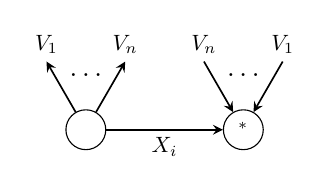
\begin{tikzpicture}[baseline=0pt]
\tikzsetup
\node[morphism] (ph) at (0,0) {$\ph$};
\node[morphism] (ph*) at (2,0) {$\ph^*$};
\node at (0,0.7) {$\dots$};
\node at (2,0.7) {$\dots$};
\draw[tikzdefault,->] (ph)-- +(120:1cm) node[pos=1.0,above,scale=0.8]
{$V_1$};
\draw[tikzdefault,->] (ph)-- +(60:1cm) node[pos=1.0,above,scale=0.8]
{$V_n$};
\draw[tikzdefault,<-] (ph*)-- +(120:1cm) node[pos=1.0,above,scale=0.8]
{$V_n$};
\draw[tikzdefault,<-] (ph*)-- +(60:1cm) node[pos=1.0,above,scale=0.8]
{$V_1$};
\draw[tikzdefault,->] (ph) -- (ph*) node[pos=0.5,below,scale=0.8] {$X_i$}; 
\end{tikzpicture}
}
%%%%%%%%%%%%%%%%%%%%%%%%%%%
\newcommand{\tzPairingIV}{
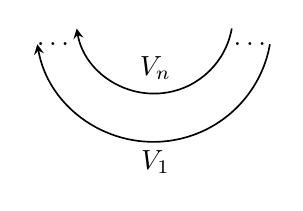
\begin{tikzpicture}[baseline=-1cm]
\tikzsetup
\node at (0.2,0) {$\dots$};
\node at (2.7,0) {$\dots$};
\draw[tikzdefault,<-] (0,0) arc(190:350:1.5cm);
 \node at(1.5,-1.5) {$V_1$};
\draw[tikzdefault,<-] (0.5,0.2) arc(190:350:1cm);
 \node at(1.5,-0.3) {$V_n$};
\end{tikzpicture}
}
%%%%%%%%%%%%%%%%%%%%%%%%%%
\newcommand{\tzPairingV}{
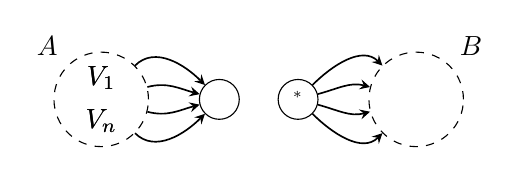
\begin{tikzpicture}[baseline=0pt]
\tikzsetup
\node[circle, draw, dashed, minimum size=1.2cm,label=135:$A$] (A) at (0,0)
{} ;
\node[morphism] (ph) at (1.5,0) {$\ph$};
\node[morphism] (ph') at (2.5,0) {$\ph^*$};
\node[circle, draw, dashed, minimum size=1.2cm, label=45:$B$] (B) at (4,0)
{};
\draw[tikzdefault, ->, out=45,in=135] (A) to (ph) 
                node[pos=0.5,above] {$V_1$};
\draw[tikzdefault, ->,out=15,in=165] (A) to (ph);
\draw[tikzdefault, ->,out=-15,in=195] (A) to (ph);
\draw[tikzdefault, ->,out=-45,in=225] (A) to (ph) 
                node[pos=0.5,below] {$V_n$};
\draw[tikzdefault, ->,out=45,in=135] (ph') to (B) 
                node[pos=0.5,above] {$V_1$};
\draw[tikzdefault, ->,out=15,in=165] (ph') to (B);
\draw[tikzdefault, ->,out=-15,in=195] (ph') to (B);
\draw[tikzdefault, ->,out=-45,in=225] (ph') to (B) 
                node[pos=0.5,below] {$V_n$};
\end{tikzpicture}
}
%%%%%%%%%%%%%%%%%%%%%%%%%%
\newcommand{\tzPairingVI}{
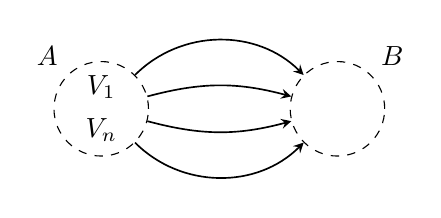
\begin{tikzpicture}[baseline=0pt]
\tikzsetup
\node[circle, draw, dashed, minimum size=1.2cm,label=135:$A$] (A) at (0,0)
{};
\node[circle, draw, dashed, minimum size=1.2cm,label=45:$B$] (B) at (3,0)
{};
\draw[tikzdefault, ->,out=45,in=135] (A) to (B) 
                node[pos=0.5,above] {$V_1$};
\draw[tikzdefault, ->,out=15,in=165] (A) to (B);
\draw[tikzdefault, ->,out=-15,in=195] (A) to (B);
\draw[tikzdefault, ->,out=-45,in=225] (A) to (B) 
                node[pos=0.5,below] {$V_n$};
\end{tikzpicture}
}
%%%%%%%%%%%%%%%%%%%%%%%%%%%
\newcommand{\tzPairingVII}{
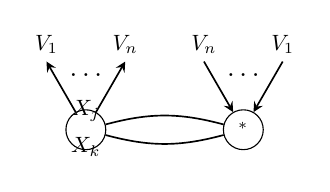
\begin{tikzpicture}[baseline=0pt]
\tikzsetup
\node[morphism] (ph) at (0,0) {$\ph$};
\node[morphism] (ph*) at (2,0) {$\ph^*$};
\node at (0,0.7) {$\dots$};
\node at (2,0.7) {$\dots$};
\draw[tikzdefault,->] (ph)-- +(120:1cm) node[pos=1.0,above,scale=0.8]
{$V_1$};
\draw[tikzdefault,->] (ph)-- +(60:1cm) node[pos=1.0,above,scale=0.8]
{$V_n$};
\draw[tikzdefault,<-] (ph*)-- +(120:1cm) node[pos=1.0,above,scale=0.8]
{$V_n$};
\draw[tikzdefault,<-] (ph*)-- +(60:1cm) node[pos=1.0,above,scale=0.8]
{$V_1$};
\draw[tikzdefault,out=15,in=165] (ph) to (ph*)
node[pos=0.5,above,scale=0.8] {$X_j$};
\draw[tikzdefault,out=-15,in=195] (ph) to (ph*)
node[pos=0.5,below,scale=0.8] {$X_k$};
\end{tikzpicture}
}


%%%%%%%%%%%%%%%%%%%%%%%%%%%
\newcommand{\tzPairingVIII}{
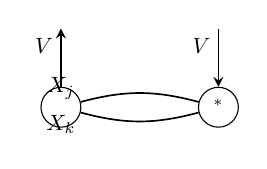
\begin{tikzpicture}[baseline=0pt]
\tikzsetup
\node[morphism] (ph) at (0,0) {$\ph$};
\node[morphism] (ph*) at (2,0) {$\ph^*$};
\draw[tikzdefault,->] (ph)-- +(90:1cm) node[pos=0.7,left,scale=0.8] {$V$};
\draw[tikzdefault,<-] (ph*)--  +(90:1cm) node[pos=0.7,left,scale=0.8]
{$V$};
\draw[tikzdefault,out=15,in=165] (ph) to (ph*)
node[pos=0.5,above,scale=0.8] {$X_j$};
\draw[tikzdefault,out=-15,in=195] (ph) to (ph*)
node[pos=0.5,below,scale=0.8]
{$X_k$};
\end{tikzpicture}
}


%%%%%%%%%%%%%%%%%%%%%%%%%%%
\newcommand{\tzPairingIX}{
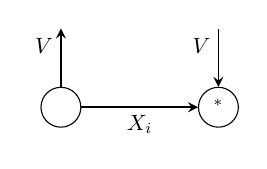
\begin{tikzpicture}[baseline=0pt]
\tikzsetup
\node[morphism] (ph) at (0,0) {$\ph$};
\node[morphism] (ph*) at (2,0) {$\ph^*$};
\draw[tikzdefault,->] (ph)-- +(90:1cm) node[pos=0.7,left,scale=0.8] {$V$};
\draw[tikzdefault,<-] (ph*)--  +(90:1cm) node[pos=0.7,left,scale=0.8]
{$V$};
\draw[tikzdefault,->] (ph) -- (ph*) node[pos=0.5,below,scale=0.8] {$X_i$};
\end{tikzpicture}
}




%%%%%%%%%%%%%%%%%%%%%%%%%%%
\newcommand{\tzSphereDiagram}{
 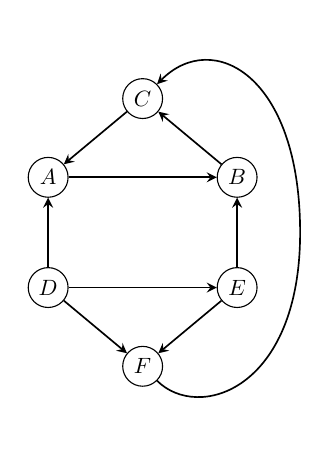
\begin{tikzpicture}[baseline=0pt]
\tikzsetup
\node[morphism] (C) at (0,1.7cm) {$C$};
\node[morphism] (A) at (-1.2cm,0.7cm) {$A$};
\node[morphism] (B) at (1.2cm,0.7cm) {$B$};
\node[morphism] (D) at (-1.2cm,-0.7cm) {$D$};
\node[morphism] (E) at (1.2cm,-0.7cm) {$E$};
\node[morphism] (F) at (0,-1.7cm) {$F$};
\begin{scope}[tikzdefault,->]
\draw (C)--(A);
\draw (A) -- (B);
\draw (B) -- (C);
\draw (D)--(A);
\draw (E)--(B);
\draw (D)--(E);
\draw (D)--(F);
\draw (E)--(F);
\draw[<-] (C.45) .. controls +(45:1cm) and +(90:2cm) .. (2,0)
.. controls +(-90:2cm) and +(-45:1cm) .. (F);
\end{scope}
\end{tikzpicture}
}
%%%%%%%%%%%%%%%%%%%%%%%%%%%
\newcommand{\tzCrossing}{
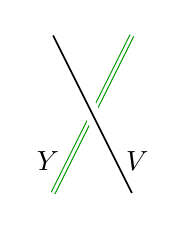
\begin{tikzpicture}[baseline=0pt]
\tikzsetup
\draw[drinfeld center](0,0)--(1cm,2cm) node [pos=0.2, left,black] {$Y$};
\draw[overline](1cm,0) -- (0,2cm) node [pos=0.2, right] {$V$};
\end{tikzpicture}
}


%%%%%%%%%%%%%%%%%%%%%%%%%%%
\newcommand{\tzProjectionI}{
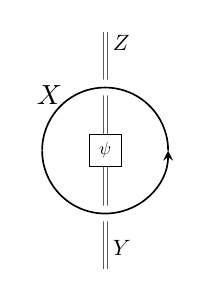
\begin{tikzpicture}[baseline=0pt]
\tikzsetup
\node[coupon,scale=0.8] (ph) at (0,0) {$\psi$};
\draw[drinfeld center](0,-1.5)--(ph) node[pos=0.2, right, black,scale=0.8]
{$Y$};
\draw[drinfeld center](ph) -- (0,1.5) node[pos=0.9, right,black, scale=0.8]
{$Z$};
  \draw[->,overline] (-0.8,0) arc (-180:0:0.8);
  \draw[-,overline] (0.8,0) arc (0:180:0.8);
\node at (135:1cm) {$X$};
\end{tikzpicture}
}
%%%%%%%%%%%%%%%%%%%%%%%%%%%
\newcommand{\tzProjectionIa}{
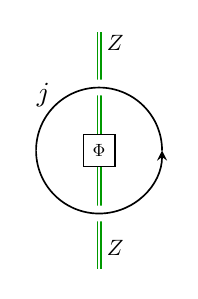
\begin{tikzpicture}[baseline=0pt]
\tikzsetup
\node[coupon,scale=0.8] (ph) at (0,0) {$\Phi$};
\draw[drinfeld center](0,-1.5)--(ph) node[pos=0.2, right, black,scale=0.8]
{$Z$};
\draw[drinfeld center](ph) -- (0,1.5) node[pos=0.9, right,black, scale=0.8]
{$Z$};
  \draw[->,overline] (-0.8,0) arc (-180:0:0.8);
  \draw[-,overline] (0.8,0) arc (0:180:0.8);
\node at (135:1cm) {$j$};
\end{tikzpicture}
}


%%%%%%%%%%%%%%%%%%%%%%%%%%%
\newcommand{\tzProjectionII}{
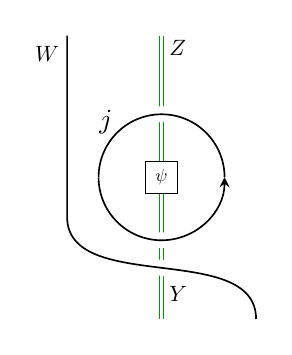
\begin{tikzpicture}[baseline=0pt]
\tikzsetup
\node[coupon,scale=0.8] (ph) at (0,0) {$\psi$};
\draw[drinfeld center](0,-1.8)--(ph) node[pos=0.2, right, black,scale=0.8]
{$Y$};
\draw[drinfeld center](ph) -- (0,1.8) node[pos=0.9, right,black, scale=0.8]
{$Z$};
  \draw[->,overline] (-0.8,0) arc (-180:0:0.8);
  \draw[-,overline] (0.8,0) arc (0:180:0.8);
\node at (135:1cm) {$j$};
\draw[overline] (1.2,-1.8) .. controls +(0cm,1cm) and +(0cm,-1cm) ..
(-1.2,-0.5)-- (-1.2,1.8) 
   node[pos=0.9,left, scale=0.8] {$W$};
\end{tikzpicture}
}

%%%%%%%%%%%%%%%%%%%%%%%%%%%
\newcommand{\tzProjectionIII}{
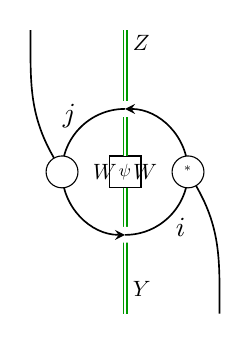
\begin{tikzpicture}[baseline=0pt]
\tikzsetup
\node[coupon,scale=0.8] (psi) at (0,0) {$\psi$};
\draw[drinfeld center](0,-1.8)--(psi) node[pos=0.2, right, black,scale=0.8]
{$Y$};
\draw[drinfeld center](psi) -- (0,1.8) node[pos=0.9, right,black,
scale=0.8]
{$Z$};
\draw[->,overline] (0,0.8) arc (90:270:0.8);
\draw[->,overline] (0,-0.8) arc (-90:90:0.8);
\node[morphism, scale=0.8,fill=white] (ph) at (-0.8,0) {$\ph$};  
\node[morphism, scale=0.8,fill=white] (ph*) at (0.8,0) {$\ph^*$};  
\node at (135:1cm) {$j$};
\node at (-45:1cm) {$i$};
\draw[tikzdefault,out=120,in=-90] (ph.120) to (-1.2,1.8)
   node[pos=0.9,left, scale=0.8] {$W$};
\draw[tikzdefault,out=-60,in=90] (ph*.-60) to (1.2,-1.8)
   node[pos=0.9,right, scale=0.8] {$W$};
\end{tikzpicture}
}




%%%%%%%%%%%%%%%%%%%%%%%%%%%
\newcommand{\tzProjectionIV}{
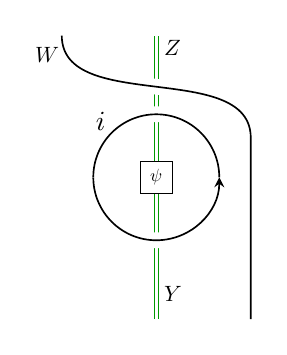
\begin{tikzpicture}[baseline=0pt]
\tikzsetup
\node[coupon,scale=0.8] (ph) at (0,0) {$\psi$};
\draw[drinfeld center](0,-1.8)--(ph) node[pos=0.2, right, black,scale=0.8]
{$Y$};
\draw[drinfeld center](ph) -- (0,1.8) node[pos=0.9, right,black, scale=0.8]
{$Z$};
  \draw[->,overline] (-0.8,0) arc (-180:0:0.8);
  \draw[-,overline] (0.8,0) arc (0:180:0.8);
\node at (135:1cm) {$i$};
\draw[overline] (1.2,-1.8) -- (1.2,0.5) 
 .. controls +(0cm,1cm) and +(0cm,-1cm) .. (-1.2,1.8) 
   node[pos=0.9,left, scale=0.8] {$W$};
\end{tikzpicture}
}





%%%%%%%%%%%%%%%%%%%%%%%%%%%
\newcommand{\tzHalfBraid}{
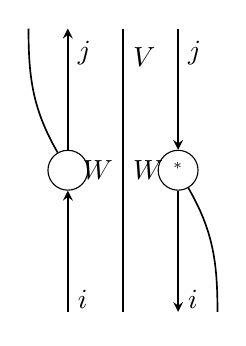
\begin{tikzpicture}[baseline=0pt]
\tikzsetup
\coordinate (bot) at (0,-1.8);
\coordinate (top) at (0,1.8);
\draw [tikzdefault] (bot)--(top) node[pos=0.9, right] {$V$};
\node[morphism] (ph) at (-0.7,0) {$\ph$};
\node[morphism] (ph*) at (0.7,0) {$\ph^*$};
\draw[tikzdefault,->] (ph|-bot) -- (ph) node[pos=0.1,right] {$i$};
\draw[tikzdefault,->] (ph) -- (ph|-top) node[pos=0.8,right] {$j$};
\draw[tikzdefault, out=120, in=-90] (ph.120) to (-1.2,1.8)
node[pos=0.8,left] {$W$};
\draw[tikzdefault,<-] (ph*|-bot) -- (ph*) node[pos=0.1,right] {$i$};
\draw[tikzdefault,<-] (ph*) -- (ph*|-top) node[pos=0.8,right] {$j$};
\draw[tikzdefault, out=-60, in=90] (ph*.-60) to (1.2,-1.8)
     node[pos=0.8,right] {$W$};
\end{tikzpicture}
}



%%%%%%%%%%%%%%%%%%%%%%%%%%%
\newcommand{\tzFunctI}{
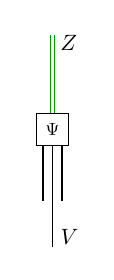
\begin{tikzpicture}[baseline=0pt]
\tikzsetup
\node[coupon,scale=0.8] (psi) at (0,0) {$\Psi$};
\draw[tikzdefault](0,-1.5)--(psi) node[pos=0.1, right, scale=0.8]
{$V$};
\draw[tikzdefault](psi.-60)-- +(0,-0.7cm) node[pos=0.8, right, scale=0.8]
{$\one$};
\draw[tikzdefault](psi.-120)-- +(0,-0.7cm) node[pos=0.8, left, scale=0.8]
{$\one$};
\draw[drinfeld center](psi) -- (0,1.2) node[pos=0.9, right,black,
scale=0.8] {$Z$};
\end{tikzpicture}
}

%%%%%%%%%%%%%%%%%%%%%%%%%%%
\newcommand{\tzFunctII}{
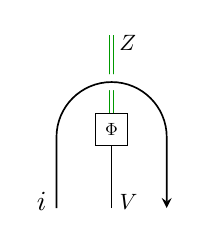
\begin{tikzpicture}[baseline=0pt]
\tikzsetup
\coordinate (V) at (0,-1);
\node[coupon,scale=0.8] (psi) at (0,0) {$\Phi$};
\draw[tikzdefault](V)--(psi) node[pos=0.1, right, scale=0.8]
{$V$};
\draw[drinfeld center](psi) -- (0,1.2) node[pos=0.9, right,black,
scale=0.8] {$Z$};
\draw[overline,->] (-0.7,-1)-- +(0,0.9) node[pos=0.1, left] {$i$} arc
(180:0:0.7cm) -- (0.7,-1);
\end{tikzpicture}
}
%%%%%%%%%%%%%%%%%%%%%%%%%%%
\newcommand{\tzFunctIII}{
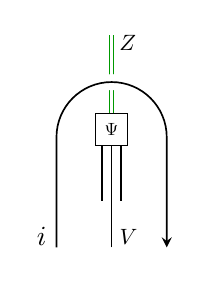
\begin{tikzpicture}[baseline=0pt]
\tikzsetup
\coordinate (V) at (0,-1.5);
\node[coupon,scale=0.8] (psi) at (0,0) {$\Psi$};
\draw[tikzdefault](V)--(psi) node[pos=0.1, right, scale=0.8]
{$V$};
\draw[drinfeld center](psi) -- (0,1.2) node[pos=0.9, right,black,
scale=0.8] {$Z$};
\draw[overline,->] (-0.7,-1.5)-- +(0,1.4) node[pos=0.1, left] {$i$} arc
(180:0:0.7cm) -- (0.7,-1.5);
\draw[tikzdefault](psi.-60)-- +(0,-0.7cm)
node[pos=0.8, right, scale=0.8]
{$\one$};
\draw[tikzdefault](psi.-120)-- +(0,-0.7cm) node[pos=0.8, left, scale=0.8]
{$\one$};

\end{tikzpicture}
}

%%%%%%%%%%%%%%%%%%%%%%%%%%%
\newcommand{\tzFunctIV}{
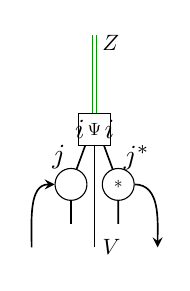
\begin{tikzpicture}[baseline=0pt]
\tikzsetup
\coordinate (V) at (0,-1.5);
\node[coupon,scale=0.8] (psi) at (0,0) {$\Psi$};
\node[morphism,scale=0.8] (ph) at (-0.3,-0.7) {$\ph$};
\node[morphism,scale=0.8] (ph*) at (0.3,-0.7) {$\ph*$};
\draw[tikzdefault](V)--(psi) node[pos=0, right, scale=0.8]
{$V$};
\draw[drinfeld center](psi) -- (0,1.2) node[pos=0.9, right,black,
scale=0.8] {$Z$};
\draw[tikzdefault,->, out=90,in=180] (-0.8,-1.5) to (ph.180) node[pos=0.1,
left] {$i$};
\draw[tikzdefault,<-, out=90,in=0] (0.8,-1.5) to (ph*.0) node[pos=0.1,
right] {$i$};
\draw[tikzdefault](psi.-60)-- (ph*) node[pos=0.5,right=2pt] {$j^*$}
  -- +(0,-0.5) node[pos=0.8, right, scale=0.8] {$\one$};
\draw[tikzdefault](psi.-120)-- (ph) node[pos=0.5,left=2pt] {$j$} 
  -- +(0,-0.5) node[pos=0.8, left, scale=0.8] {$\one$};
\end{tikzpicture}
}

%%%%%%%%%%%%%%%%%%%%%%%%%%%
\newcommand{\tzFunctV}{
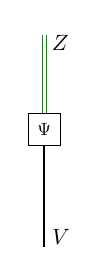
\begin{tikzpicture}[baseline=0pt]
\tikzsetup
\coordinate (V) at (0,-1.5);
\node[coupon,scale=0.8] (psi) at (0,0) {$\Psi$};
\draw[tikzdefault](V)--(psi) node[pos=0.1, right, scale=0.8]
{$V$};
\draw[drinfeld center](psi) -- (0,1.2) node[pos=0.9, right,black,
scale=0.8] {$Z$};
\end{tikzpicture}
}

%%%%%%%%%%%%%%%%%%%%%%%%%%%
\newcommand{\tzSphereDiagramII}{
 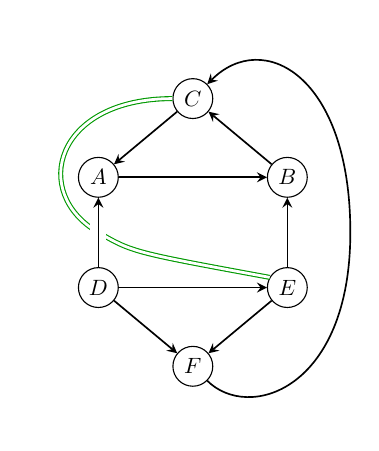
\begin{tikzpicture}[baseline=0pt]
\tikzsetup
\node[morphism] (C) at (0,1.7cm) {$C$};
\node[morphism] (A) at (-1.2cm,0.7cm) {$A$};
\node[morphism] (B) at (1.2cm,0.7cm) {$B$};
\node[morphism] (D) at (-1.2cm,-0.7cm) {$D$};
\node[morphism] (E) at (1.2cm,-0.7cm) {$E$};
\node[morphism] (F) at (0,-1.7cm) {$F$};
\begin{scope}[tikzdefault,->]
\draw (C)--(A);
\draw (A) -- (B);
\draw (B) -- (C);
\draw (E)--(B);
\draw (D)--(E);
\draw (D)--(F);
\draw (E)--(F);
\draw[<-] (C.45) .. controls +(45:1cm) and +(90:2cm) .. (2,0)
.. controls +(-90:2cm) and +(-45:1cm) .. (F);
\end{scope}
\draw[drinfeld center]
   (C.180) .. controls +(180:1.5cm) and +(150:1cm) ..
   (-1.2cm,0) .. controls +(-30:0.5cm) .. (E.150);
\draw[overline,->] (D)--(A);
\end{tikzpicture}
}

%%%%%%%%%%%%%%%%%%%%%%%%%%%
\newcommand{\tzHomotopyI}{
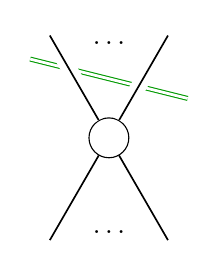
\begin{tikzpicture}[baseline=0pt]
\tikzsetup
\node[morphism] (ph) at (0,0) {$\ph$};
\node at (0,1.2) {$\dots$};
\node at (0,-1.2) {$\dots$};
\draw[drinfeld center] (-1,1)--(1,0.5);
\draw[overline] (ph)-- +(120:1.5cm);
\draw[overline] (ph)-- +(60:1.5cm);
\draw[tikzdefault] (ph)-- +(-120:1.5cm);
\draw[tikzdefault] (ph)-- +(-60:1.5cm);
\end{tikzpicture}
}

%%%%%%%%%%%%%%%%%%%%%%%%%%%
\newcommand{\tzHomotopyII}{
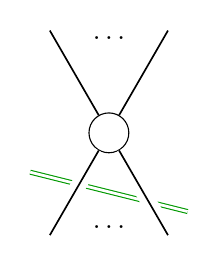
\begin{tikzpicture}[baseline=0pt]
\tikzsetup
\node[morphism] (ph) at (0,0) {$\ph$};
\node at (0,1.2) {$\dots$};
\node at (0,-1.2) {$\dots$};
\draw[drinfeld center] (-1,-0.5)--(1,-1);
\draw[tikzdefault] (ph)-- +(120:1.5cm);
\draw[tikzdefault] (ph)-- +(60:1.5cm);
\draw[overline] (ph)-- +(-120:1.5cm);
\draw[overline] (ph)-- +(-60:1.5cm);
\end{tikzpicture}
}




%%%%%%%%%%%%%%%%%%%%%%%%%%%
\newcommand{\tzStateSpaceI}{
   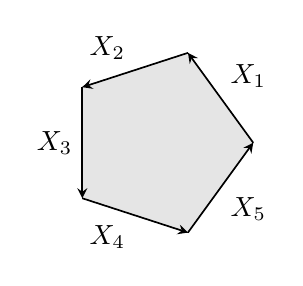
\begin{tikzpicture}[baseline=0pt]
   \tikzsetup
   \coordinate (a0) at (0:1.2cm);
   \coordinate (a1) at (72:1.2cm);
   \coordinate (a2) at (144:1.2cm);
   \coordinate (a3) at (216:1.2cm);
   \coordinate (a4) at (288:1.2cm);
  \fill[cell] (a0)--(a1)--(a2)--(a3)--(a4)--(a0);
  \draw[tikzdefault,->] (a0)--(a1) node [pos=0.5,auto=right] {$X_1$};
  \draw[tikzdefault,->] (a1)--(a2) node [pos=0.5,auto=right] {$X_2$};
  \draw[tikzdefault,->] (a2)--(a3) node [pos=0.5,auto=right] {$X_3$};
  \draw[tikzdefault,->] (a3)--(a4) node [pos=0.5,auto=right] {$X_4$};
  \draw[tikzdefault,->] (a4)--(a0) node [pos=0.5,auto=right] {$X_5$};
   \end{tikzpicture}
}


%%%%%%%%%%%%%%%%%%%%%%%%%%%
\newcommand{\tzStateSpaceII}{
   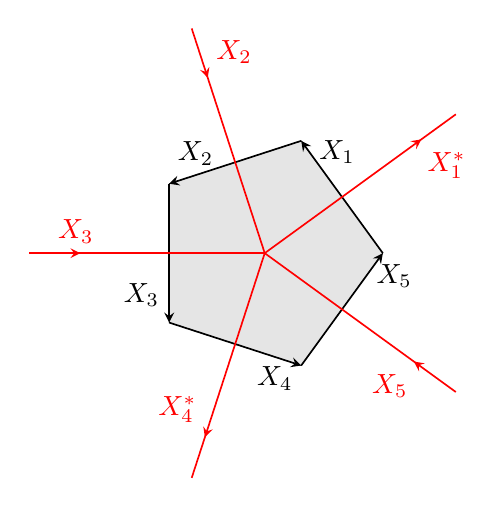
\begin{tikzpicture}[baseline=0pt]
   \tikzsetup
   \coordinate (a0) at (0:1.5cm);
   \coordinate (a1) at (72:1.5cm);
   \coordinate (a2) at (144:1.5cm);
   \coordinate (a3) at (216:1.5cm);
   \coordinate (a4) at (288:1.5cm);
  \fill[cell] (a0)--(a1)--(a2)--(a3)--(a4)--(a0);
  \draw[tikzdefault,->] (a0)--(a1) node [pos=0.9,right] {$X_1$};
  \draw[tikzdefault,->] (a1)--(a2) node [pos=0.8,above] {$X_2$};
  \draw[tikzdefault,->] (a2)--(a3) node [pos=0.8,left] {$X_3$};
  \draw[tikzdefault,->] (a3)--(a4) node [pos=0.8,below] {$X_4$};
  \draw[tikzdefault,->] (a4)--(a0) node [pos=0.8,right] {$X_5$};
  \draw[tikzdefault,red] (0,0) -- node[midarrow,pos=0.8]{} (36:3cm)
         node [pos=0.8,auto=right] {$X_1^*$};
  \draw[tikzdefault,red] (0,0) -- node[revmidarrow,pos=0.8]{} (108:3cm)
         node [pos=0.8,auto=right] {$X_2$};
  \draw[tikzdefault,red] (0,0) -- node[revmidarrow,pos=0.8]{} (180:3cm)
         node [pos=0.8,auto=right] {$X_3$};
  \draw[tikzdefault,red] (0,0) -- node[midarrow,pos=0.8]{} (252:3cm)
         node [pos=0.8,auto=right] {$X_4^*$};
  \draw[tikzdefault,red] (0,0) -- node[revmidarrow,pos=0.8]{} (324:3cm)
         node [pos=0.8,auto=right] {$X_5$};
   \end{tikzpicture}\qquad
   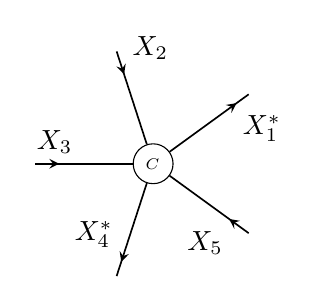
\begin{tikzpicture}[baseline=0pt]
   \tikzsetup
   \node[morphism] (ph) at (0,0) {$\ph_C$};
  \draw[tikzdefault] (ph) -- node[midarrow,pos=0.8]{} (36:1.5cm)
         node [pos=0.8,auto=right] {$X_1^*$};
  \draw[tikzdefault] (ph) -- node[revmidarrow,pos=0.8]{} (108:1.5cm)
         node [pos=0.8,auto=right] {$X_2$};
  \draw[tikzdefault] (ph) -- node[revmidarrow,pos=0.8]{} (180:1.5cm)
         node [pos=0.8,auto=right] {$X_3$};
  \draw[tikzdefault] (ph) -- node[midarrow,pos=0.8]{} (252:1.5cm)
         node [pos=0.8,auto=right] {$X_4^*$};
  \draw[tikzdefault] (ph) -- node[revmidarrow,pos=0.8]{} (324:1.5cm)
         node [pos=0.8,auto=right] {$X_5$};
\end{tikzpicture}
}


%%%%%%%%%%%%%%%%%%%%%%%%%%%
\newcommand{\tzGluingAxiomI}{
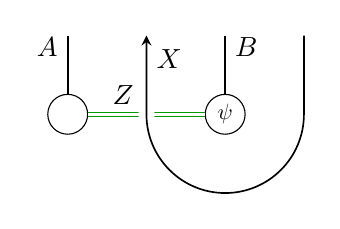
\begin{tikzpicture}[baseline=0pt]
\tikzsetup
\node[morphism] (ph) at (0,0) {$\ph$};
\node[morphism] (psi) at (2,0) {$\psi$};
\draw[tikzdefault] (ph) -- +(0,1cm) node[pos=0.8, left] {$A$};
\draw[tikzdefault] (psi) -- +(0,1cm) node[pos=0.8, right] {$B$};
\draw[drinfeld center] (ph)--(psi) node[pos=0.3,above,black]{$Z$};
\draw[->,overline](3,1)--(3,0) arc (0:-180:1cm) -- +(0,1)
node[pos=0.7,right] {$X$};
\end{tikzpicture}
}



%%%%%%%%%%%%%%%%%%%%%%%%%%
\newcommand{\tzSphereProofI}{
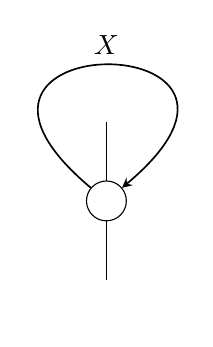
\begin{tikzpicture}[baseline=0cm]
\tikzsetup
%%%% nodes
\path[use as bounding box] (-1,-1.5) rectangle (1,2.2);
\node[morphism] (phi) at (0,0) {$\ph$};
%%%%% vertical
\draw[tikzdefault] (phi)-- +(0,1) node[pos=0.6,right=-1pt] {$\one$};
\draw[tikzdefault] (phi)-- +(0,-1) node[pos=0.6,right=-1pt] {$\one$};
%%%%% arc
\draw[tikzdefault,->] (phi).. controls +(140:3.5cm) and +(40:3.5cm) ..
(phi) node[pos=0.5,above] {$X$};
\end{tikzpicture}
}
%%%%%%%%%%%%%%%%%%%%%%%%%%
\newcommand{\tzSphereProofII}{
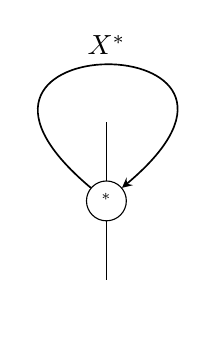
\begin{tikzpicture}[baseline=0cm]
\tikzsetup
%%%% nodes
\path[use as bounding box] (-1,-1.5) rectangle (1,2.2);
\node[morphism] (phi) at (0,0) {$\ph^*$};
%%%%% vertical
\draw[tikzdefault] (phi)-- +(0,1) node[pos=0.6,right=-1pt] {$\one$};
\draw[tikzdefault] (phi)-- +(0,-1) node[pos=0.6,right=-1pt] {$\one$};
%%%%% arc
\draw[tikzdefault,->] (phi).. controls +(140:3.5cm) and +(40:3.5cm) ..
(phi) node[pos=0.5,above] {$X^*$};
\end{tikzpicture}
}

%%%%%%%%%%%%%%%%%%%%%%%%%%
\newcommand{\tzSphereProofIII}{
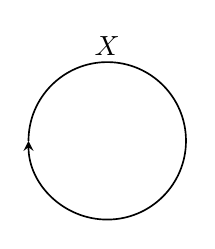
\begin{tikzpicture}[baseline=0cm]
\tikzsetup
\OrientedCircle[xscale=-1]
\node at (0,1.2) {$X$};
\end{tikzpicture}
}

%%%%%%%%%%%%%%%%%%%%%%%%%%
\newcommand{\tzSphereProofIV}{
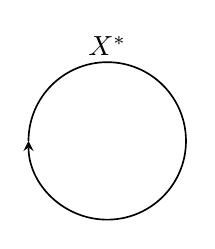
\begin{tikzpicture}[baseline=0cm]
\tikzsetup
\OrientedCircle[xscale=-1]
\node at (0,1.2) {$X^*$};
\end{tikzpicture}
}




%%%%%%%%%%%%%%%%%%%%%%%%%%%
\newcommand{\tzMoveMtwoI}{
\begin{tikzpicture}[baseline=0pt]
\tikzsetup
\node[morphism] (ph) at (0,0) {$\ph_\al$};
\node[morphism] (psi) at (2,0) {$\psi_\be$};
\node at (0,0.7) {$\dots$};
\node at (2,0.7) {$\dots$};
\draw[tikzdefault,->] (ph)-- +(120:1cm) node[pos=1.0,above,scale=0.8]
{$V_1$};
\draw[tikzdefault,->] (ph)-- +(60:1cm) node[pos=1.0,above,scale=0.8]
{$V_n$};
\draw[tikzdefault,<-] (psi)-- +(120:1cm) node[pos=1.0,above,scale=0.8]
{$W_m$};
\draw[tikzdefault,<-] (psi)-- +(60:1cm) node[pos=1.0,above,scale=0.8]
{$W_1$};
\draw[tikzdefault,->] (ph) -- (psi) node[pos=0.5,below,scale=0.8] {$X_i$}; 
\end{tikzpicture}
}

%%%%%%%%%%%%%%%%%%%%%%%%%%%
\newcommand{\tzMoveMtwoII}{
\begin{tikzpicture}[baseline=0pt]
\tikzsetup
\node[morphism] (ph) at (2,0) {$\ph^\al$};
\node[morphism] (psi) at (0,0) {$\psi^\be$};
\node at (0,0.7) {$\dots$};
\node at (2,0.7) {$\dots$};
\draw[tikzdefault,<-] (ph)-- +(120:1cm) node[pos=1.0,above,scale=0.8]
{$V_n$};
\draw[tikzdefault,<-] (ph)-- +(60:1cm) node[pos=1.0,above,scale=0.8]
{$V_1$};
\draw[tikzdefault,->] (psi)-- +(120:1cm) node[pos=1.0,above,scale=0.8]
{$W_1$};
\draw[tikzdefault,->] (psi)-- +(60:1cm) node[pos=1.0,above,scale=0.8]
{$W_m$};
\draw[tikzdefault,->] (psi) -- (ph) node[pos=0.5,below,scale=0.8] {$X^*_i$}; 
\end{tikzpicture}
}



%%%%%%%%%%%%%%%%%%%%%%%%%%%
\newcommand{\tzMoveMtwoIII}{
\begin{tikzpicture}[baseline=0pt]
\tikzsetup
\node[coupon] (ph) at (0,0) {$\ph_\al\ccc{X_i}\psi_\be$};
\draw[tikzdefault,->] (ph.150)-- +(110:1cm) node[pos=1.0,above left,scale=0.8]
{$V_1$};
\draw[tikzdefault,->] (ph.130)-- +(110:1cm) node[pos=1.0,above,scale=0.8]
{$V_n$};
\draw[tikzdefault,<-] (ph.50)-- +(70:1cm) node[pos=1.0,above,scale=0.8]
{$W_m$};
\draw[tikzdefault,<-] (ph.30)-- +(70:1cm) node[pos=1.0,above right,scale=0.8]
{$W_1$};
\end{tikzpicture}
}
%%%%%%%%%%%%%%%%%%%%%%%%%%%
\newcommand{\tzMoveMtwoIV}{
\begin{tikzpicture}[baseline=0pt]
\tikzsetup
\node[coupon] (ph) at (0,0) {$\psi^\be\ccc{X_i}\ph^\al$};
\draw[tikzdefault,<-] (ph.150)-- +(110:1cm) node[pos=1.0,above left,scale=0.8]
{$W_1$};
\draw[tikzdefault,<-] (ph.130)-- +(110:1cm) node[pos=1.0,above,scale=0.8]
{$W_m$};
\draw[tikzdefault,->] (ph.50)-- +(70:1cm) node[pos=1.0,above,scale=0.8]
{$V_m$};
\draw[tikzdefault,->] (ph.30)-- +(70:1cm) node[pos=1.0,above right,scale=0.8]
{$V_n$};
\end{tikzpicture}
}



%%%%%%%%%%%%%%%%%%%%%%%%%%
\newcommand{\tzGluingI}{
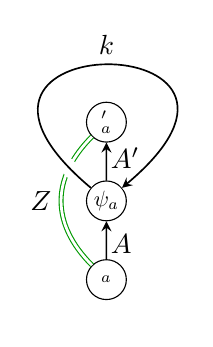
\begin{tikzpicture}[baseline=0cm]
\tikzsetup
%%%% nodes
\path[use as bounding box] (-1,-1.5) rectangle (1,2.2);
\node[morphism] (psi) at (0,0) {$\psi_a$};
\node[morphism] (ph') at (0,1) {$\ph'_a$};
\node[morphism] (ph) at (0,-1) {$\ph_a$};
%%%%%% horiz lines
\draw[drinfeld center] (ph)
               .. controls +(135:1cm) and +(-135:1cm) ..
               (ph') node[pos=0.5, left, black] {$Z$};
%%%%% vertical
\draw[tikzdefault,->] (psi)--(ph') node[pos=0.6,right=-2pt] {$A'$};
\draw[tikzdefault,->] (ph)--(psi) node[pos=0.4,right=-2pt] {$A$};
%%%%% arc
\draw[overline,->] (psi).. controls +(140:3.5cm) and +(40:3.5cm) ..
(psi) node[pos=0.5,above] {$k$};
\end{tikzpicture}
}


%%%%%%%%%%%%%%%%%%%%%%%%%%
\newcommand{\tzGluingII}{
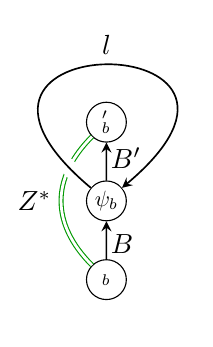
\begin{tikzpicture}[baseline=0cm]
\tikzsetup
%%%% nodes
\path[use as bounding box] (-1,-1.5) rectangle (1,2.2);
\node[morphism] (psi) at (0,0) {$\psi_b$};
\node[morphism] (ph') at (0,1) {$\ph'_b$};
\node[morphism] (ph) at (0,-1) {$\ph_b$};
%%%%%% horiz lines
\draw[drinfeld center] (ph)
               .. controls +(135:1cm) and +(-135:1cm) ..
               (ph') node[pos=0.5, left, black] {$Z^*$};
%%%%% vertical
\draw[tikzdefault,->] (psi)--(ph') node[pos=0.6,right=-2pt] {$B'$};
\draw[tikzdefault,->] (ph)--(psi) node[pos=0.4,right=-2pt] {$B$};
%%%%% arc
\draw[overline,->] (psi).. controls +(140:3.5cm) and +(40:3.5cm) ..
(psi) node[pos=0.5,above] {$l$};
\end{tikzpicture}
}




%%%%%%%%%%%%%%%%%%%%%%%%%%%
\newcommand{\tzGluingIII}{
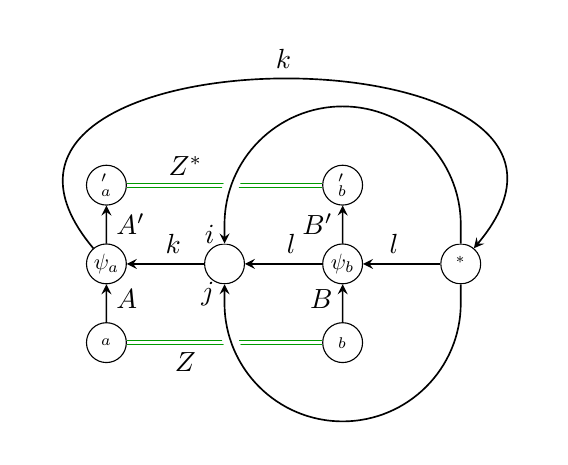
\begin{tikzpicture}[baseline=0cm]
\tikzsetup
\path[use as bounding box] (-1,-2.2) rectangle (5.5,3);
%%%% nodes
\node[morphism] (psi_a) at (0,0) {$\psi_a$};
\node[morphism] (C) at (1.5,0) {$\ph$};
\node[morphism] (psi_b) at (3,0) {$\psi_b$};
\node[morphism] (Cbar) at (4.5,0) {$\ph^*$};
\node[morphism] (ph_a') at (0,1) {$\ph'_a$};
\node[morphism] (ph_b') at (3,1) {$\ph'_b$};
\node[morphism] (ph_a) at (0,-1) {$\ph_a$};
\node[morphism] (ph_b) at (3,-1) {$\ph_b$};
%%%%%% horiz lines
\draw[drinfeld center] (ph_a)--(ph_b) node[pos=0.3,below, black] {$Z$};
\draw[drinfeld center] (ph_a')--(ph_b') node[pos=0.3,above, black] {$Z^*$};
\draw[tikzdefault,<-] (psi_a)-- (C) node[pos=0.6,above] {$k$} ;
\draw[tikzdefault,<-] (C)--(psi_b) node[pos=0.6,above] {$l$};
\draw[tikzdefault, <-] (psi_b)--(Cbar) node[pos=0.4,above] {$l$};
%%%%% to top 
\draw[tikzdefault,->] (psi_a)--(ph_a') node[pos=0.5,right] {$A'$};
\draw[tikzdefault,->] (psi_b)--(ph_b') node[pos=0.5,left] {$B'$};
\draw[overline, <-] (C)--node[left] {$i$} +(0,0.5) arc (180:0:1.5cm) -- (Cbar);
%%%%% to bottom
\draw[tikzdefault,<-] (psi_a)--(ph_a) node[pos=0.4,right] {$A$};
\draw[tikzdefault,<-] (psi_b)--(ph_b) node[pos=0.4,left] {$B$};
\draw[overline, <-] (C)--node[left] {$j$} +(0,-0.5) arc (180:360:1.5cm) -- (Cbar);
%%%%% arc
\draw[tikzdefault,->] (psi_a).. controls +(130:4cm) and +(50:4cm) ..
(Cbar) node[pos=0.5,above] {$k$};
\end{tikzpicture}
}



%%%%%%%%%%%%%%%%%%%%%%%%%%%
\newcommand{\tzGluingIV}{
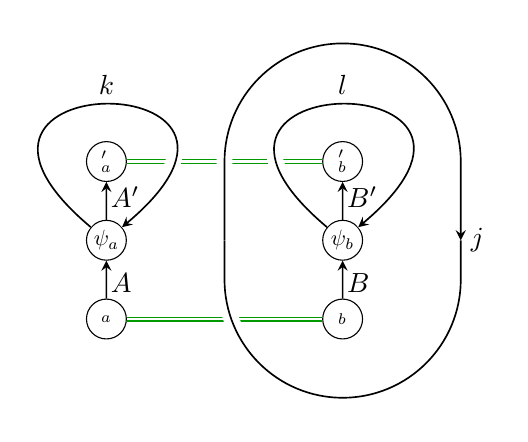
\begin{tikzpicture}[baseline=0cm]
\tikzsetup
\path[use as bounding box] (-1,-2.2) rectangle (5,2.7);

%%%% nodes
\node[morphism] (C_L) at (0,0) {$\psi_a$};
\coordinate (C) at (1.5,0);
\node[morphism] (C_R) at (3,0) {$\psi_b$};
\coordinate (Cbar) at (4.5,0);
\node[morphism] (psi_al') at (0,1) {$\ph'_a$};
\node[morphism] (psi_be') at (3,1) {$\ph'_b$};
\node[morphism] (psi_al) at (0,-1) {$\ph_a$};
\node[morphism] (psi_be) at (3,-1) {$\ph_b$};
%%%%%% horiz lines
\draw[drinfeld center] (psi_al)--(psi_be);
\draw[drinfeld center] (psi_al')--(psi_be');
%%%%% to top
\draw[tikzdefault,->] (C_L)--(psi_al') node[pos=0.6,right=-2pt] {$A'$};
\draw[tikzdefault,->] (C_R)--(psi_be') node[pos=0.6,right=-2pt] {$B'$};
\draw[overline,->] (C)-- +(0,1) arc (180:0:1.5cm) -- (Cbar)  node[right] {$j$};
%%%%% to bottom
\draw[tikzdefault,<-] (C_L)--(psi_al) node[pos=0.6,right=-2pt] {$A$};
\draw[tikzdefault,<-] (C_R)--(psi_be) node[pos=0.6,right=-2pt] {$B$};
\draw[overline] (C)-- +(0,-0.5) arc (180:360:1.5cm) -- (Cbar);
%%%%% arcs
\draw[overline,->] (C_L).. controls +(140:3.5cm) and +(40:3.5cm) ..
(C_L)  node[pos=0.5,above] {$k$};
\draw[overline,->] (C_R).. controls +(140:3.5cm) and +(40:3.5cm) ..
(C_R) node[pos=0.5,above] {$l$};
\end{tikzpicture}
}








%%%%%%%%%%%%%%%%%%%%%%%%%%%
\newcommand{\tzGluingV}{
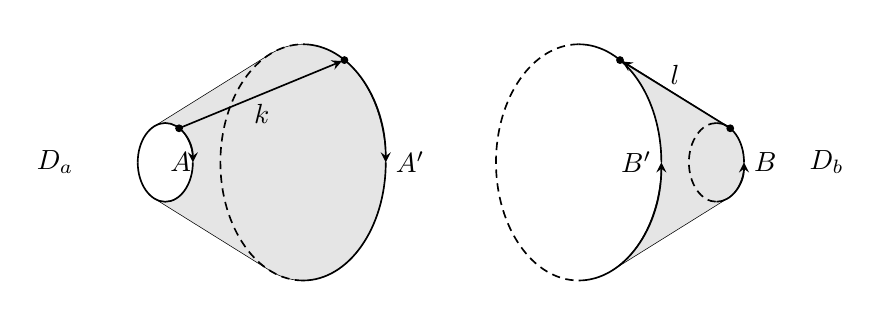
\begin{tikzpicture}
\tikzsetup

%%%%%%
\begin{scope}[tikzdefault,xscale=0.7]
\coordinate (a1) at (60:0.5cm);\coordinate (a2) at ($(10cm,0)+(60:0.5cm)$);
\coordinate (b1) at ($(2.5cm,0)+(60:1.5cm)$);\coordinate (b2) at ($(7.5cm,0)+(60:1.5cm)$);
\coordinate (c1) at (0,-0.5);\coordinate (c2) at (10,-0.5);
\coordinate (d1) at (2.5,-1.5);\coordinate (d2) at (7.5,-1.5);


\path[cell] (114:0.5cm)--
             ($(2.5cm,0)+(114:1.5cm)$)
            arc (114:-114:1.5cm)
            --  (-114:0.5cm)
            arc (-114:114:0.5cm);
\path[cell] ($(10cm,0)+(66:0.5cm)$)--
             ($(7.5cm,0)+(66:1.5cm)$)
            arc (66:-66:1.5cm)
            --  ($(10cm,0)+(-66:0.5cm)$)
            arc (-66:66:0.5cm);


\node[dotnode]  at (a1) {};
\node[dotnode]  at (b1) {};
\node[dotnode]  at (a2) {};
\node[dotnode]  at (b2) {};
%%%%% left inner circle
\OrientedCircle[xscale=0.5, yscale=-0.5] \node[left=-3pt]  at (0.5,0)  {$A$};
\node at (-2,0) {$D_a$};
%%%%% left outer circle
\HalfDashedOrientedCircle[ xshift=2.5cm, xscale=1.5, yscale=-1.5] \node[right]  at (4,0)  {$A'$};
%%%%%% vertical lines
\draw[->,shorten > = 1pt] (a1)-- node[below] {$k$}(b1);
\draw[->,shorten > = 1pt] (a2)-- node[above] {$l$}(b2);
%%%%% right inner circle
\HalfDashedOrientedCircle[xshift=10cm,scale=0.5] 
  \node[right]  at (10.5,0) {$B$};
  \node at (12,0) {$D_b$};
%%%%% right outer circle
\HalfDashedOrientedCircle[xshift=7.5cm,scale=1.5] 
  \node[left]  at (9,0) {$B'$};

\end{scope}
\end{tikzpicture}
}





%%%%%%%%%%%%%%%%%%%%%%%%%%%
\newcommand{\tzGluingVI}{
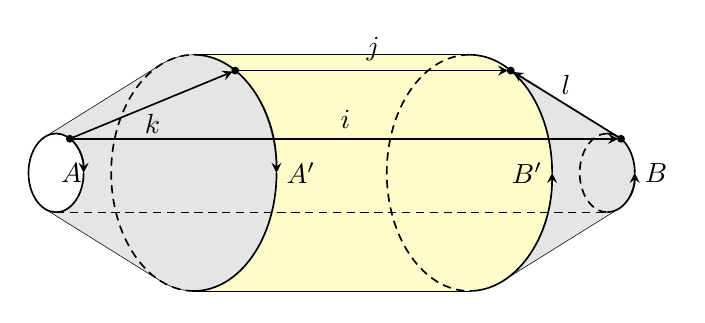
\begin{tikzpicture}
\tikzsetup

%%%%%%
\begin{scope}[tikzdefault,xscale=0.7]
\coordinate (a1) at (60:0.5cm);\coordinate (a2) at ($(10cm,0)+(60:0.5cm)$);
\coordinate (b1) at ($(2.5cm,0)+(60:1.5cm)$);\coordinate (b2) at ($(7.5cm,0)+(60:1.5cm)$);
\coordinate (c1) at (0,-0.5);\coordinate (c2) at (10,-0.5);
\coordinate (d1) at (2.5,-1.5);\coordinate (d2) at (7.5,-1.5);


\path[cell] (114:0.5cm)--
             ($(2.5cm,0)+(114:1.5cm)$)
            arc (114:-114:1.5cm)
            --  (-114:0.5cm)
            arc (-114:114:0.5cm);
\path[cell] ($(10cm,0)+(66:0.5cm)$)--
             ($(7.5cm,0)+(66:1.5cm)$)
            arc (66:-66:1.5cm)
            --  ($(10cm,0)+(-66:0.5cm)$)
            arc (-66:66:0.5cm);

\fill[yellow!20] (d1) arc (-90:90:1.5) -- (7.5,1.5) arc (90:-90:1.5)--cycle;


\node[dotnode]  at (a1) {};
\node[dotnode]  at (b1) {};
\node[dotnode]  at (a2) {};
\node[dotnode]  at (b2) {};
%%%%% left inner circle
\OrientedCircle[xscale=0.5, yscale=-0.5] \node[left=-3pt]  at (0.5,0)  {$A$};
%%%%% left outer circle
\HalfDashedOrientedCircle[ xshift=2.5cm, xscale=1.5, yscale=-1.5] \node[right]  at (4,0)  {$A'$};
%%%%% horizontal lines 
\draw[->,shorten > = 1pt] (a1)--node [above] {$i$}(a2);
\draw[->,shorten > = 1pt] (b1)--node [above] {$j$}(b2);
\draw[thin,densely dashed] (c1)--(c2);
\draw[very thin] (d1)--(d2);
\draw[very thin] (2.5,1.5)--(7.5,1.5);
%%%%%% vertical lines
\draw[->,shorten > = 1pt] (a1)-- node[below] {$k$}(b1);
\draw[->,shorten > = 1pt] (a2)-- node[above] {$l$}(b2);
%%%%% right inner circle
\HalfDashedOrientedCircle[xshift=10cm,scale=0.5] 
  \node[right]  at (10.5,0) {$B$};
%%%%% right outer circle
\HalfDashedOrientedCircle[xshift=7.5cm,scale=1.5] 
  \node[left]  at (9,0) {$B'$};

\end{scope}
\end{tikzpicture}
}






%%%%%%%%%%%%%%%%%%%%%%%%%%%
\newcommand{\tzCylinderI}{
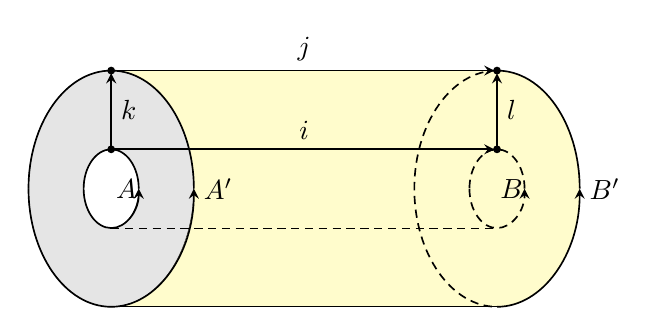
\begin{tikzpicture}
\tikzsetup

%%%%%%
\begin{scope}[tikzdefault,xscale=0.7]
\coordinate (a1) at (0,0.5);\coordinate (a2) at (7,0.5);
\coordinate (b1) at (0,1.5);\coordinate (b2) at (7,1.5);
\coordinate (c1) at (0,-0.5);\coordinate (c2) at (7,-0.5);
\coordinate (d1) at (0,-1.5);\coordinate (d2) at (7,-1.5);


\path[cell] (a1) arc(-270:89.9:0.5) -- ++(0,1) arc
(89.9:-270:1.5)--cycle;

\fill[yellow!20] (d1) arc (-90:90:1.5) -- (b2) arc (90:-90:1.5)--cycle;


\node[dotnode]  at (a1) {};
\node[dotnode]  at (b1) {};
\node[dotnode]  at (a2) {};
\node[dotnode]  at (b2) {};
%%%%% left inner circle
\OrientedCircle[scale=0.5] \node[left=-3pt]  at (0.5,0)  {$A$};
%%%%% left outer circle
\OrientedCircle[scale=1.5] \node[right]  at (1.5,0)  {$A'$};
%%%%% horizontal lines 
\draw[->,shorten > = 1pt] (a1)--node [above] {$i$}(a2);
\draw[->,shorten > = 1pt] (b1)--node [above] {$j$}(b2);
\draw[thin,densely dashed] (c1)--(c2);
\draw[thin] (d1)--(d2);
%%%%%% vertical lines
\draw[->,shorten > = 1pt] (a1)-- node[right] {$k$}(b1);
\draw[->,shorten > = 1pt] (a2)-- node[right] {$l$}(b2);
%%%%% right inner circle
\OrientedCircle[xshift=7cm,scale=0.5,densely dashed] 
  \node[left=-3pt]  at (7.5,0) {$B$};
%%%%% right inner circle
\HalfDashedOrientedCircle[xshift=7cm,scale=1.5] 
  \node[right]  at (8.5,0) {$B'$};

\end{scope}
\end{tikzpicture}
}

%%%%%%%%%%%%%%%%%%%%%%%%%%%
\newcommand{\tzCL}{
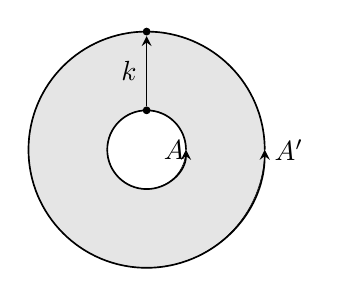
\begin{tikzpicture}[baseline]
\tikzsetup
\path[cell, even odd rule] (0,0) circle (0.5) (0,0) circle (1.5); 
\OrientedCircle[scale=0.5] 
        \node[left=-3pt] at (0.5,0) {$A$};
\OrientedCircle[scale=1.5] 
        \node[right] at (1.5,0) {$A'$};
\node[dotnode]  (a1) at (0,0.5){};
\node[dotnode]  (a2) at (0,1.5){};
\draw[->,tikzdefault] (a1) -- node[left] {$k$} (a2);
\end{tikzpicture}
}

%%%%%%%%%%%%%%%%%%%%%%%%%%%
\newcommand{\tzCR}{
\begin{tikzpicture}[baseline]
\tikzsetup
\path[cell, even odd rule] (0,0) circle (0.5) (0,0) circle (1.5); 
\OrientedCircle[xscale=-0.5, yscale=0.5] 
        \node[right=-3pt] at (-0.5,0) {$B$};
\OrientedCircle[xscale=-1.5,yscale=1.5] 
        \node[left] at (-1.5,0) {$B'$};
\node[dotnode]  (b1) at (0,0.5){};
\node[dotnode]  (b2) at (0,1.5){};
\draw[->,tikzdefault] (a1) -- node[left] {$l$} (a2);
\end{tikzpicture}
}

%%%%%%%%%%%%%%%%%%%%%%%%%%%
\newcommand{\tzCin}{
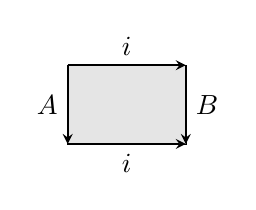
\begin{tikzpicture}[baseline=0.5cm]
\tikzsetup
\coordinate (a) at (0,0);\coordinate (b) at (0,1);
\coordinate (c) at (1.5,1);\coordinate (d) at (1.5,0);
\path[cell] (a)--(b)--(c)--(d)--cycle;
\draw[tikzdefault,<-] (a)-- node [left] {$A$} (b);
\draw[tikzdefault,->] (b)-- node [above] {$i$} (c);
\draw[tikzdefault,<-] (d)-- node [right] {$B$} (c);
\draw[tikzdefault,->] (a)-- node [below] {$i$} (d);
\end{tikzpicture}
}
%%%%%%%%%%%%%%%%%%%%%%%%%%%
\newcommand{\tzCout}{
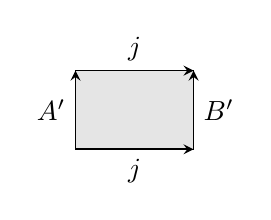
\begin{tikzpicture}[baseline=0.5cm]
\tikzsetup
\coordinate (a) at (0,0);\coordinate (b) at (0,1);
\coordinate (c) at (1.5,1);\coordinate (d) at (1.5,0);
\path[cell] (a)--(b)--(c)--(d)--cycle;
\draw[tikzdefault,->] (a)-- node [left] {$A'$} (b);
\draw[tikzdefault,->] (b)-- node [above] {$j$} (c);
\draw[tikzdefault,->] (d)-- node [right] {$B'$} (c);
\draw[tikzdefault,->] (a)-- node [below] {$j$} (d);
\end{tikzpicture}
}
%%%%%%%%%%%%%%%%%%%%%%%%%%%
\newcommand{\tzC}{
\begin{tikzpicture}[baseline=0.5cm]
\tikzsetup
\coordinate (a) at (0,0);\coordinate (b) at (0,1);
\coordinate (c) at (1.5,1);\coordinate (d) at (1.5,0);
\path[cell] (a)--(b)--(c)--(d)--cycle;
\draw[tikzdefault,->] (a)-- node [left] {$k$} (b);
\draw[tikzdefault,->] (b)-- node [above] {$j$} (c);
\draw[tikzdefault,->] (d)-- node [right] {$l$} (c);
\draw[tikzdefault,->] (a)-- node [below] {$i$} (d);
\end{tikzpicture}}
%%%%%%%%%%%%%%%%%%%%%%%%%%%
\newcommand{\tzCube}{
\begin{tikzpicture}[baseline=0.5cm]
\tikzsetup
\coordinate (a1) at (0,0);\coordinate (b1) at (1.2,1);
\coordinate (d1) at (2,0);\coordinate (c1) at (3.2,1);
\coordinate (a2) at (0,2);\coordinate (b2) at (1.2,3);
\coordinate (d2) at (2,2);\coordinate (c2) at (3.2,3);
% back square
\draw[tikzdefault,->] (b1)-- (c1) node [pos=0.8,above] {$i$} ;
\draw[tikzdefault,->] (b2)-- node [above] {$j$} (c2);
\draw[tikzdefault,->] (b1)-- (b2) node [pos=0.3,left] {$k$};
\draw[tikzdefault,->] (c1)-- node [right] {$l$} (c2);
% front square 
\draw[overline] (a2)-- (d2) node [pos=0.8, above] {$j$} ;
\draw[overline,->] (d1)-- (d2) node [pos=0.7,right] {$l$};
\draw[tikzdefault,->] (a2)-- (d2); 
\draw[tikzdefault,->] (a1)-- (a2)node [pos=0.3,left] {$k$};
\draw[tikzdefault,->] (a1)--  (d1) node [pos=0.6,above] {$i$};
% remaining lines
\draw[tikzdefault,->] (a2)--  (b2) node [pos=0.7,left]{$A'$};
\draw[tikzdefault,->] (a1)--  (b1) node [pos=0.7,left] {$A$};
\draw[tikzdefault,->] (d1)-- (c1) node [pos=0.3,right] {$B$};
\draw[tikzdefault,->] (d2)-- (c2) node[pos=0.3,right] {$B'$};
\end{tikzpicture}
}
%%%%%%%%%%%%%%%%%%%%%%%%%%%
\newcommand{\tzDualGraphCyl}{
\begin{tikzpicture}[baseline=0.5cm]
\tikzsetup
\node[dotnode, label={left:$C_L$}] (C_L) at (0,0) {};
\node[dotnode, label={above right:$C$}] (C) at (2,0) {};
\node[dotnode, label={above right:$C_R$}] (C_R) at (4,0) {};
\node[dotnode, label={right:$\ov{C}$}] (Cbar) at (6,0) {};
\node[dotnode, label={above:$C_{out}$}] (C_out) at (3,2) {};
\node[dotnode, label={below:$C_{in}$}] (C_in) at (3,-2) {};
\draw[tikzdefault] (C_L)--(C)--(C_R)--(Cbar);
\draw[tikzdefault] (C_in)--(C_L)--(C_out);
\draw[tikzdefault] (C_in)--(C)--(C_out);
\draw[tikzdefault] (C_in)--(C_R)--(C_out);
\draw[tikzdefault] (C_in)--(Cbar)--(C_out);
\draw[tikzdefault] (C_L).. controls +(90:4cm) and +(90:4cm) .. (Cbar);
\end{tikzpicture}
}
%%%%%%%%%%%%%%%%%%%%%%%%%%%
\newcommand{\tzDualGraphCylII}{
\begin{tikzpicture}[baseline=0.5cm]
\tikzsetup
%%%% nodes
\node[morphism] (C_L) at (0,0) {$\psi_a$};
\node[morphism] (C) at (2,0) {$\ph$};
\node[morphism] (C_R) at (4,0) {$\psi_b$};
\node[morphism] (Cbar) at (6,0) {$\ph'$};
\node[morphism] (C_out) at (3,3) {$\psi_{out}$};
\node[morphism] (C_in) at (3,-3) {$\psi_{in}$};
%%%%%% horiz lines
\draw[tikzdefault,<-] (C_L)-- (C) node[pos=0.6,above] {$k$} ;
\draw[tikzdefault,<-] (C)--(C_R) node[pos=0.6,above] {$l$};
\draw[tikzdefault, <-] (C_R)--(Cbar) node[pos=0.4,above] {$l$};
%%%%% to top (C_out)
\draw[tikzdefault,<-] (C_L)--(C_out) node[pos=0.4,left=2pt] {$A'$};
\draw[tikzdefault,<-] (C)--(C_out) node[pos=0.4,left] {$j$};
\draw[tikzdefault,->] (C_R)--(C_out) node[pos=0.4,right] {$B'$};
\draw[tikzdefault,->] (Cbar)--(C_out) node[pos=0.4,right=3pt] {$j$};
%%%%% to bottom (C_in)
\draw[tikzdefault,<-] (C_in)--(C_L) node[pos=0.6,left=2pt] {$A$};
\draw[tikzdefault,->] (C_in)--(C) node[pos=0.6,left] {$i$};
\draw[tikzdefault,->] (C_in)--(C_R) node[pos=0.6,right] {$B$};
\draw[tikzdefault,<-] (C_in)--(Cbar) node[pos=0.6,right=3pt] {$i$};
%%%%% arc
\draw[tikzdefault,->] (C_L).. controls +(90:5cm) and +(90:5cm) .. (Cbar);
\node at (3,4.2) {$k$};
\end{tikzpicture}
}
%%%%%%%%%%%%%%%%%%%%%%%%%%%
\newcommand{\tzNsphereI}{
\begin{tikzpicture}[baseline=0cm]
\tikzsetup
\draw (0,-1.5) rectangle (7,-2.2); \coordinate (bot) at (0,-1.5);
\draw (0,1.5) rectangle (7,2.2);\coordinate (top) at (0,1.5); 
\node at (3.5, -1.8) {$\ph_0$};
\node at (3.5, 1.8) {$\ph'_0$};
\node[morphism,scale=0.8] (X_1) at (0.3,0) {$\al_1$};
\node[morphism, scale=0.8] (V_1) at (1,0) {$\beta_1$};
\node[morphism, scale=0.8] (X_1*) at (1.7,0){$\al_1^*$};
\node[morphism, scale=0.8] (X_n) at (5.3,0) {$\al_n$};
\node[morphism, scale=0.8] (V_n) at (6,0) {$\beta_n$};
\node[morphism, scale=0.8] (X_n*) at (6.7,0) {$\al_n^*$};
%%%%%%%%%%%% vertical lines
\draw[->,tikzdefault] (X_1|-bot) -- (X_1) 
                  node[pos=0.5,left=-1pt,scale=0.7]{$i_1$};
 \draw[->,tikzdefault] (X_1)--(X_1|-top)
                  node[pos=0.5,left=-1pt,scale=0.7]{$j_1$};;
\draw[->,tikzdefault] (V_1|-bot) -- (V_1) 
                  node[pos=0.5,left=-1pt,scale=0.7]{$U_1$};
 \draw[->,tikzdefault] (V_1) -- (V_1|-top) 
                  node[pos=0.5,left=-1pt,scale=0.7]{$V_1$};
\draw[<-,tikzdefault] (X_1*|-bot) -- (X_1*) 
                  node[pos=0.5,right=-1pt,scale=0.7]{$i_1$};
 \draw[<-,tikzdefault] (X_1*) --(X_1*|-top) 
                  node[pos=0.5,right=-1pt,scale=0.7]{$j_1$};
\draw[->,tikzdefault] (X_n|-bot) -- (X_n) 
                  node[pos=0.5,left=-1pt,scale=0.7]{$i_n$};
\draw[->,tikzdefault] (X_n)--(X_n|-top) 
                  node[pos=0.5,left=-1pt,scale=0.7]{$j_n$};
\draw[->,tikzdefault] (V_n|-bot) -- (V_n) 
                  node[pos=0.5,left=-1pt,scale=0.7]{$U_n$};
\draw[->,tikzdefault] (V_n) --(V_n|-top) 
                  node[pos=0.5,left=-1pt,scale=0.7]{$V_n$};
\draw[<-,tikzdefault] (X_n*|-bot) -- (X_n*) 
                  node[pos=0.5,right=-1pt,scale=0.7]{$i_n$};
\draw[<-,tikzdefault] (X_n*) --(X_n*|-top) 
                  node[pos=0.5,right=-1pt,scale=0.7]{$j_n$};
%%%%%%%%%%%% horizontal lines
\draw[->,tikzdefault] (X_1)-- (V_1);
\draw[->,tikzdefault] (V_1)-- (X_1*);
\draw[->,tikzdefault] (X_1*)-- +(0:0.7cm)
              node[pos=0.8,above,scale=0.7]{$l$};
\draw[<-,tikzdefault] (X_n)-- +(180:0.7cm)
              node[pos=0.8,above,scale=0.7]{$l$};
\draw[->,tikzdefault] (X_n)-- (V_n);
\draw[->,tikzdefault] (V_n)-- (X_n*);
%%%%%%%%%%%% the circle
\draw[<-,tikzdefault] (X_1.west) arc (90:270:1.3cm)
               node[pos=0.5,above left=1pt , scale=0.7] {$l$} 
               coordinate (leftbot);
\draw[->,tikzdefault] (X_n*.east) arc (90:-90:1.3cm)  coordinate
(rightbot);
\draw[<-,tikzdefault] (leftbot)--(rightbot);
\end{tikzpicture}
}
%%%%%%%%%%%%%%%%%%%%%%%%%%%
\newcommand{\tzNsphereII}{
\begin{tikzpicture}[baseline=3cm]
\tikzsetup
\node[morphism] (Y_1bot) at (0,1.5) {$\ph_i$};
\node[morphism] (Y_1side) at (0,3) {$\be_i^*$};
\node[morphism] (Y_1top) at (0,4.5) {$\ph'_i$};
\draw[tikzdefault,->] (Y_1bot)--(Y_1side) 
               node[midway, left,scale=0.8] {$U_i$};
\draw[tikzdefault,->] (Y_1side)--(Y_1top) 
               node[midway, left,scale=0.8] {$V_i$};
\draw[drinfeld center] (Y_1bot) .. 
      controls +(45:1cm) and +(-45:1cm) 
      ..(Y_1top) node[pos=0.3, right,scale=0.8] {$Y_i$};
\draw[tikzdefault,overline] 
 (Y_1side.east) 
    .. controls +(0:1.5cm) and + (0:1.5cm) ..
 (0,5.5) node [pos=0.5,right, scale=0.8] {$k_i$}
.. controls +(180:1.5cm) and + (180:1.5cm).. 
 (Y_1side.west);
\end{tikzpicture}
}
%%%%%%%%%%%%%%%%%%%%%%%%%%%
\newcommand{\tzNsphereIII}{
\begin{tikzpicture}[baseline=0cm]
\tikzsetup
\draw (0,-1.5) rectangle (7,-2.2); \coordinate (bot) at (0,-1.5);
\draw (0,1.5) rectangle (7,2.2);\coordinate (top) at (0,1.5); 
\node at (3.5, -1.8) {$\ph_0$};
\node at (3.5, 1.8) {$\ph'_0$};
\node[morphism,scale=0.8] (X_1) at (0.3,0) {$\al_1$};
\node[morphism, scale=0.8] (V_1bot) at (1,-0.7) {$\ph_1$};
\node[morphism, scale=0.8] (V_1top) at (1,0.7) {$\ph'_1$};
\node[morphism, scale=0.8] (X_1*) at (1.7,0){$\al_1^*$};
\node[morphism, scale=0.8] (X_n) at (5.3,0) {$\al_n$};
\node[morphism, scale=0.8] (V_nbot) at (6,-0.7) {$\ph_n$};
\node[morphism, scale=0.8] (V_ntop) at (6,0.7) {$\ph'_n$};
\node[morphism, scale=0.8] (X_n*) at (6.7,0) {$\al_n^*$};
%%%%%%%%%%%% vertical lines
\draw[->,tikzdefault] (X_1|-bot) -- (X_1) 
                  node[pos=0.5,left=-1pt,scale=0.7]{$i_1$};
 \draw[->,tikzdefault] (X_1)--(X_1|-top)
                  node[pos=0.5,left=-1pt,scale=0.7]{$j_1$};;
\draw[->,tikzdefault] (V_1bot|-bot) -- (V_1bot) 
                  node[pos=0.5,left=-1pt,scale=0.7]{$U_1$};
\draw[drinfeld center] (V_1bot) -- (V_1top) 
                  node[pos=0.5,left=-1pt,scale=0.7]{$Y_1$};
 \draw[->,tikzdefault] (V_1top) -- (V_1top|-top) 
                  node[pos=0.5,left=-1pt,scale=0.7]{$V_1$};
\draw[<-,tikzdefault] (X_1*|-bot) -- (X_1*) 
                  node[pos=0.5,right=-1pt,scale=0.7]{$i_1$};
 \draw[<-,tikzdefault] (X_1*) --(X_1*|-top) 
                  node[pos=0.5,right=-1pt,scale=0.7]{$j_1$};
\draw[->,tikzdefault] (X_n|-bot) -- (X_n) 
                  node[pos=0.5,left=-1pt,scale=0.7]{$i_n$};
\draw[<-,tikzdefault] (X_n)--(X_n|-top) 
                  node[pos=0.5,left=-1pt,scale=0.7]{$j_n$};
\draw[->,tikzdefault] (V_nbot|-bot) -- (V_nbot) 
                  node[pos=0.5,left=-1pt,scale=0.7]{$U_n$};
\draw[->,tikzdefault] (V_ntop) --(V_ntop|-top) 
                  node[pos=0.5,left=-1pt,scale=0.7]{$V_n$};
\draw[drinfeld center] (V_nbot) -- (V_ntop) 
                  node[pos=0.5,left=-1pt,scale=0.7]{$Y_1$};
\draw[<-,tikzdefault] (X_n*|-bot) -- (X_n*) 
                  node[pos=0.5,right=-1pt,scale=0.7]{$i_n$};
\draw[->,tikzdefault] (X_n*) --(X_n*|-top) 
                  node[pos=0.5,right=-1pt,scale=0.7]{$j_n$};
%%%%%%%%%%%% horizontal lines
\draw[->,overline] (X_1)-- (X_1*) node[pos=0.3, above,scale=0.8] {$k_1$};
\draw[->,tikzdefault] (X_1*)-- +(0:0.7cm)
              node[pos=0.8,above,scale=0.7]{$l$};
\draw[<-,tikzdefault] (X_n)-- +(180:0.7cm)
              node[pos=0.8,above,scale=0.7]{$l$};
\draw[->,overline] (X_n)-- (X_n*) node[pos=0.3, above,scale=0.8] {$k_n$};
%%%%%%%%%%%% the circle
\draw[<-,tikzdefault] (X_1.west) arc (90:270:1.3cm)
               node[pos=0.5,above left=1pt , scale=0.7] {$l$} 
               coordinate (leftbot);
\draw[->,tikzdefault] (X_n*.east) arc (90:-90:1.3cm)  coordinate
(rightbot);
\draw[<-,tikzdefault] (leftbot)--(rightbot);
\end{tikzpicture}
}

%%%%%%%%%%%%%%%%%%%%%%%%%%%
\newcommand{\tzNsphereIV}{
\begin{tikzpicture}[baseline=0cm]
\tikzsetup
\coordinate (bot) at (0,-1.5);
\coordinate (top) at (0,1.5); 
\node at (3.5, -1.8) {$\ph$};
\node at (3.5, 1.8) {$\ph'$};
\coordinate (X_1) at (0.3,0);
\coordinate (V_1) at (1,0);
\coordinate (X_1*) at (1.7,0);
\coordinate (X_n) at (5.3,0);
\coordinate (V_n) at (6,0);
\coordinate (X_n*) at (6.7,0);
%%%%%%%%%%%% vertical lines
\draw[drinfeld center] (V_1|-bot) -- (V_1|-top) 
                  node[pos=0.1,left=-1pt,scale=0.7,black]{$Y_1$};
\draw[drinfeld center] (V_n|-bot) -- (V_n|-top) 
                  node[pos=0.1,left=-1pt,scale=0.7,black]{$Y_n$};
%%%%%%%%%%%% arcs
\draw[->,overline] (X_1|-bot) -- node[pos=0.9,left,scale=0.8]{$i_1$} 
                  +(0,0.3cm) arc (180:0:0.7cm) -- (X_1*|-bot);
\draw[<-,overline] (X_1|-top) -- node[pos=0.9,left,scale=0.8]{$j_1$}
                  +(0,-0.3cm) arc (180:360:0.7cm) -- (X_1*|-top);
\draw[->,overline] (X_n|-bot) -- node[pos=0.9,left,scale=0.8]{$i_n$} 
                  +(0,0.3cm) arc (180:0:0.7cm) -- (X_n*|-bot);
\draw[<-,overline] (X_n|-top) -- node[pos=0.9,left,scale=0.8]{$j_n$}
                  +(0,-0.3cm) arc (180:360:0.7cm) -- (X_n*|-top);
%%%%%%%%%%%% horizontal lines
\draw[overline] (X_1)--(X_n*) node[pos=0.5, above,scale=0.8] {$l$};
%%%%%%%%%%%% the circle
\draw[<-,tikzdefault] (X_1) arc (90:270:1.3cm)
               coordinate (rightbot)
               node[pos=0.5,above left=1pt , scale=0.7] {$l$};
\draw[->,tikzdefault] (X_n*) arc (90:-90:1.3cm) coordinate (rightbot);
\draw[tikzdefault] (leftbot)--(rightbot);
\draw (0,-1.5) rectangle (7,-2.2);
\draw (0,1.5) rectangle (7,2.2);
\node at (3.5, -1) {$\dots$};
\node at (3.5, 1) {$\dots$};
\end{tikzpicture}
}
%%%%%%%%%%%%%%%%%%%%%%%%%%%
\newcommand{\tzNsphereV}{
\begin{tikzpicture}[baseline=0cm]
\tikzsetup
\coordinate (bot) at (0,-1.5);
\coordinate (top) at (0,1.5); 
\node at (3.5, -1.8) {$\ph$};
\coordinate (X_1) at (0.3,0);
\coordinate (V_1) at (1,0);
\coordinate (X_1*) at (1.7,0);
\coordinate (X_n) at (5.3,0);
\coordinate (V_n) at (6,0);
\coordinate (X_n*) at (6.7,0);
%%%%%%%%%%%% vertical lines
\draw[drinfeld center] (V_1|-bot) -- (V_1|-top) 
                  node[pos=0.1,left=-1pt,scale=0.7,black]{$Y_1$};
\draw[drinfeld center] (V_n|-bot) -- (V_n|-top) 
                  node[pos=0.1,left=-1pt,scale=0.7,black]{$Y_n$};
%%%%%%%%%%%% arcs
\draw[->,overline] (X_1|-bot) -- node[pos=0.9,left,scale=0.8]{$i_1$} 
                  +(0,0.3cm) arc (180:0:0.7cm) -- (X_1*|-bot);
\draw[<-,overline] (X_1|-top) -- node[pos=0.9,left,scale=0.8]{$j_1$}
                  +(0,-0.3cm) arc (180:360:0.7cm) -- (X_1*|-top);
\draw[->,overline] (X_n|-bot) -- node[pos=0.9,left,scale=0.8]{$i_n$} 
                  +(0,0.3cm) arc (180:0:0.7cm) -- (X_n*|-bot);
\draw[<-,overline] (X_n|-top) -- node[pos=0.9,left,scale=0.8]{$j_n$}
                  +(0,-0.3cm) arc (180:360:0.7cm) -- (X_n*|-top);
%%%%%%%%%%%% horizontal lines
\draw[overline] (X_1)--(X_n*) node[pos=0.5, above,scale=0.8] {$l$};
%%%%%%%%%%%% the circle
\draw[<-,tikzdefault] (X_1) arc (90:270:1.3cm)
               coordinate (leftbot)
               node[pos=0.5,above left=1pt , scale=0.7] {$l$};
\draw[->,tikzdefault] (X_n*) arc (90:-90:1.3cm) coordinate (rightbot);
\draw[tikzdefault] (leftbot)--(rightbot);
\draw (0,-1.5) rectangle (7,-2.2);
\node at (3.5, -1) {$\dots$};
\end{tikzpicture}
}
%%%%%%%%%%%%%%%%%%%%%%%%%%%
\newcommand{\tzNsphereVI}{
\begin{tikzpicture}[baseline=0cm]
\tikzsetup
\coordinate (bot) at (0,-1);
\coordinate (top) at (0,1); 
\node at (3.5, -1.3) {$\psi$};
\coordinate (X_1) at (0.3,0);
\coordinate (V_1) at (1,0);
\coordinate (X_1*) at (1.7,0);
\coordinate (X_n) at (5.3,0);
\coordinate (V_n) at (6,0);
\coordinate (X_n*) at (6.7,0);
%%%%%%%%%%%% vertical lines
\draw[drinfeld center] (V_1|-bot) -- (V_1|-top) 
                  node[pos=0.1,left=-1pt,scale=0.7,black]{$Y_1$};
\draw[drinfeld center] (V_n|-bot) -- (V_n|-top) 
                  node[pos=0.1,left=-1pt,scale=0.7,black]{$Y_n$};
%%%%%%%%%%%% arcs
\draw[<-,overline] (X_1|-top) -- node[pos=0.9,left,scale=0.8]{$j_1$}
                  +(0,-0.3cm) arc (180:360:0.7cm) -- (X_1*|-top);
\draw[<-,overline] (X_n|-top) -- node[pos=0.9,left,scale=0.8]{$j_n$}
                  +(0,-0.3cm) arc (180:360:0.7cm) -- (X_n*|-top);
%%%%%%%%%%%
\draw (0,-1) rectangle (7,-1.7);
\node at (3.5, -0.5) {$\dots$};
\end{tikzpicture}
}
%%%%%%%%%%%%%%%%%%%%%%%%%%%
%\newcommand{\tz}{
%}
